\documentclass[letterpaper]{article}
\usepackage[utf8]{inputenc}
\usepackage[spanish]{babel}
\usepackage{amssymb, amsmath}
\usepackage{graphicx}
\usepackage{lipsum}
\usepackage{dsfont}
\usepackage[margin=1.5cm,
vmargin={1.5cm,1.3cm},
includefoot]{geometry}
\usepackage{setspace}
\usepackage{subcaption}
\usepackage{tocloft}
\usepackage{upgreek}
\usepackage{amsthm}
\usepackage{graphicx}
\usepackage{paralist}
\usepackage{fancyhdr}
\usepackage{lmodern}
\usepackage{tcolorbox}
\usepackage{color}
\usepackage{tikz}
\tcbuselibrary{skins,breakable}
\pagestyle{fancy}

\renewcommand{\headrulewidth}{0.4pt}
\renewcommand{\footrulewidth}{0.4pt}

\providecommand{\abs}[1]{\lvert#1\rvert}
\providecommand{\norm}[1]{\lVert#1\rVert}														  
\newcommand{\V}{\mathds{V}}

\newcommand{\W}{\mathds{W}}

\newcommand{\F}{\mathds{F}}

\newcommand{\tq}{ \quad \cdot  \backepsilon \cdot \quad }

\newcommand{\ld}{\lim\limits_{x \to 0^{+}}}

\newcommand{\li}{\lim\limits_{x \to 0^{-}}}

\newcommand{\la}{\lim\limits_{x \to a}}

\newcommand{\R}{\mathds{R}}

\newcommand{\Po}{\mathds{P}_2(\mathds{R})}

\renewcommand{\*}{\cdot}

\makeatletter
\renewcommand*\env@matrix[1][*\c@MaxMatrixCols c]{%
	\hskip -\arraycolsep
	\let\@ifnextchar\new@ifnextchar
	\array{#1}}
\makeatother

\newtheorem{theorem}{Teorema}[section]
\theoremstyle{definition}
\newtheorem{definition}{Definición}
              		   
\begin{document}

\setlength{\unitlength}{1cm}
\thispagestyle{empty}
\begin{picture}(19,3)
\put(-0.5,1.2){
\includegraphics[scale=.20]{unam1.png}}
\put(16,1){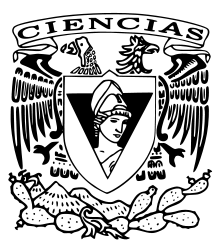
\includegraphics[scale=.29]{fciencias1.png}}
\end{picture}

\begin{center}
\vspace{-114pt}
\textbf{\large Matemáticas para las Ciencias II}\\
\textbf{ Semestre 2020-2}\\
Prof. Pedro Porras Flores\\
Ayud. Irving Hernández Rosas \\
\textbf{Tarea-examen I}\\[0.2cm]
Kevin Ariel Merino Peña\footnote{317031326}\\ [0.2cm]
\end{center}
\vspace{-10pt}
\rule{19cm}{0.3mm}

\vspace{0.5cm}
\noindent Realice los siguientes ejercicios, escribiendo el procedimiento claramente. Y recuerden que la tarea-examen se entrega individual. 

\noindent1. Muestre que $\mathbb{P}_{2}(\mathbb{R}) = \{ c  + bx + ax^2  \,  \vert \, a,b,c \in \mathbb{R} \}$, es un espacio vectorial con la suma usual y la multiplicación por escalar usual, es decir:
\begin{align*}
     + \colon & \mathbb{P}_{2}(\mathbb{R}) \times \mathbb{P}_{2}(\mathbb{R}) \longrightarrow \mathbb{P}_{2}(\mathbb{R}) \\
    & (a_1 x^2 + b_1x + c_1 , a_2 x^2 + b_2x + c_2) \mapsto  (a_1 + a_2)x^2 + (b_1 + b_2)x + (c_1 + c_2). \\
    \mu \colon & \mathbb{R} \times \mathbb{P}_{2}(\mathbb{R}) \longrightarrow \mathbb{P}_{2}(\mathbb{R}) \\
    & (\alpha, (a_1 x^2 + b_1x + c_1)) \mapsto  (\alpha a_1)x^2 + (\alpha b_1)x + (\alpha c_1).
 \end{align*}
\begin{definition}
	Sea $ \V $ un conjunto no vacío con 2 operaciones definidas $ (+,\mu) $ y un campo $ \F = \R $ que cumple
	\begin{enumerate}
		\item Sean $ \vec{x}, \vec{y} \in \V $, entonces $ \vec{x} + \vec{y} = \vec{y} + \vec{x} $
		\item Sean $ \vec{x}, \vec{y}, \vec{z} \in \V $, entonces
		$ (\vec{x} + \vec{y}) + \vec{z} = \vec{x} + (\vec{y} + \vec{z}) $
		\item Existe $ \vec{0} \in \V \tq \vec{0} + \vec{x} = \vec{x}, \qquad \forall \vec{x} \in \V$
		\item Para todo $ \vec{x} \in \V $ existe $ \vec{y} \in \V $ tal que $ \vec{x} + \vec{y} = 0 $
		\item Para todo $ \vec{x} \in \V $ se cumple que $ \vec{1} \vec{x} = \vec{x} $ donde $ \vec{1} $ es el neutro multiplicativo de $ \F(\R) $
		\item Para todo $ \alpha, \beta \in \F $ y $ \vec{x} \in \V $ se cumple $ (\alpha\beta)\vec{x} = \alpha(\beta \vec{x}) $
		\item Para todo $ \alpha, \beta  \in \F$ y $ \vec{x} \in \V $ entonces $ (\alpha + \beta)\vec{x} = \alpha\vec{x} + \beta\vec{x} $
		\item Sea $ \alpha \in \F $ y $ \vec{x}, \vec{y} \in \V $, entonces $ \alpha(\vec{x} + \vec{y}) = \alpha\vec{x} + \alpha\vec{y} $
	\end{enumerate}
\end{definition}
Sean $ \vec{x}, \vec{y} \in \Po $, por demostrar $\vec{x} + \vec{y} = \vec{y} + \vec{x}  $, como los elementos de $ \Po $ son de la forma $ c + ax + bx^2$, entonces digamos que \[ \vec{x} = a_1 + a_2x + a_3x^2 \] \[ \vec{y} = b_1 + b_2x + b_3x^2 \]
\begin{align*}
	\vec{x} + \vec{y} &=  (a_1 + a_2x + a_3x^2) + (b_1 + b_2x + b_3x^2) && \text{Por definición de los vectores}\\
	\vec{x} + \vec{y} &=  (a_1 + b_1) + (a_2 + b_2)x + (a_3 + b_3)x^2&& \text{Por definición de la suma}\\
	\vec{x} + \vec{y} &=  (b_1 + a_1) + (b_2 + a_2)x + (b_3 + a_3)x^2&& \text{Porque los elementos en $ \R $ conmutan}\\
	\vec{x} + \vec{y} &=  (b_1 + b_2x + b_3x^2) + (a_1 + a_2x + a_3x^2) && \text{Por la definición de +}\\
	\vec{x} + \vec{y} &=  \vec{y} + \vec{x}&& \text{Por definición de los vectores}\\
\end{align*}
\begin{center}
	$ \therefore $ los elementos de $ \Po $ conmutan, \textit{i.e.} $ \vec{x} + \vec{y} = 	\vec{y} + \vec{x} $
\end{center}

Sean $ \vec{x}, \vec{y}, \vec{z} \in \V $ por demostrar $  (\vec{x} + \vec{y}) + \vec{z} = \vec{x} + (\vec{y} + \vec{z})$
como los elementos de $ \Po $ son de la forma $ c + ax + bx^2$, entonces digamos que \[ \vec{x} = a_1 + a_2x + a_3x^2 \] \[ \vec{y} = b_1 + b_2x + b_3x^2 \] \[ \vec{z} = c_1 + c_2x + c_3x^2 \]

\begin{align*}
	(\vec{x} + \vec{y}) + \vec{z} &= ( a_1 + a_2x + a_3x^2 + b_1 + b_2x + b_3x^2) + c_1 + c_2x + c_3x^2&& \text{Por definición de los vectores}\\
	(\vec{x} + \vec{y}) + \vec{z} &= ( (a_1 + b_1)  + (a_2 + b_2)x + (a_3 + b_3) x^2 ) + c_1 + c_2x + c_3x^2&& \text{Por definición de los + en $ \Po $}\\ 
	(\vec{x} + \vec{y}) + \vec{z} &= ((a_1 + b_1) + c_1)  + ((a_2 + b_2) + c_2 )x + ((a_3 + b_3) + c_3) x^2 && \text{Por definición de los + en $ \Po $}\\ 
	(\vec{x} + \vec{y}) + \vec{z} &= (a_1 + (b_1 + c_1))  + (a_2 + (b_2 + c_2))x + (a_3 + (b_3 + c_3)) x^2 && \text{Porque en $ \R $ la suma es asociativa}\\ 
	(\vec{x} + \vec{y}) + \vec{z} &= a_1 + (b_1 + c_1)  + a_2x + (b_2 + c_2)x + a_3x^2 + (b_3 + c_3)x^2 && \text{Emplendo la definición de suma}\\ 
	(\vec{x} + \vec{y}) + \vec{z} &= a_1 + (b_1 + c_1)  + a_2x + (b_2x + c_2x) + a_3x^2 + (b_3x^2 + c_3x^2) && \text{Aplicando distrubutividad}\\ 
	(\vec{x} + \vec{y}) + \vec{z} &= \vec{x} + (\vec{y} + \vec{z}) && \text{Definiendo la suma en $ \Po $}\\ 
\end{align*}
\begin{center}
	$ \therefore \qquad $ la suma es asociativa en $ \Po $
\end{center}

Por demostrar: $ \vec{0} + \vec{x} = \vec{x} $. Proponemos $ \vec{0} = 0 + 0x + 0x^2 $. \\
Sea $ \vec{x} \in \V $, entonces $ \vec{x} $ es de la forma \[ \vec{x} = a_1 + a_2x + a_3x^2  \]
\begin{align*}
	\vec{0} + \vec{x} &=  (0 + 0x + 0x^2) + (a_1 + a_2x + a_3x^2 )  && \text{ Por definición de $ \vec{x}, \vec{0} $}\\
	\vec{0} + \vec{x} &=  (0 + a_1) + (0 + a_2)x + (0 + a_3)x^2 && \text{ Por definición de  + en $ \Po $}\\
	\vec{0} + \vec{x} &=  a_1 +  a_2x + a_3x^2 && \text{ Porque los elementos en $ \R $ tienen neutro aditivo}\\
	\vec{0} + \vec{x} &= \vec{x} && \text{ Por definición de $ \vec{x} $}
\end{align*}
\begin{center}
	$ \therefore   \qquad 0 + 0x + 0x^2 $ es el neutro adivito en $ \Po $
\end{center}

Sea $ \vec{x} \in \V $, por demostrar, existe $ \vec{y} \in V  \tq \vec{x} +  \vec{y} = \vec{0}$, sabemos que  los elementos de $ \V $ tienen la siguiente forma\[  \vec{x} = a_1 + a_2x + a_3x^2 \] proponemos \[ \vec{y} = -a_1 - a_2x - a_3x^2 \]
\begin{align*}
	\vec{x} +  \vec{y} &= (a_1 + a_2x + a_3x^2) + (-a_1 - a_2x - a_3x^2 )&& \text{Por definición de los vectores}\\
	\vec{x} +  \vec{y} &= (a_1 - a_1) + (a_2 - a_2)x + (a_3 - a_3)x^2&& \text{Por definición de la suma en $ \Po $}\\
	\vec{x} +  \vec{y} &= (0) + (0)x + (0)x^2&& \text{Los elementos del campo tienen inverso aditivo}\\
	\vec{x} +  \vec{y} &= \vec{0}&& \text{Por definición del neutro aditivo}
\end{align*}
\begin{center}
	$ \therefore \qquad -a_1 - a_2x - a_3x^2  $ es el inverso aditivo de $ \vec{x} $
\end{center}

Sea $ \vec{x}  \in \V $, por demostrar $ \vec{1} \* \vec{x} = \vec{x}$\\ Proponemos $ \vec{1} = 1 $
\begin{align*}
	1\* \vec{x} &= 1(a_1 + a_2x + a_3x^2) && \text{Por definición de los elementos de $ \Po $}\\
	1\* \vec{x} &= (1 \* a_1) + (1 \* a_2)x + (1 \* a_3)x^2 && \text{Por  definición del producto en $ \Po $}\\
	1\* \vec{x} &= a_1 + a_2x + a_3x^2 && \text{Puesto que los elementos del campo tienen neutro multiplicativo}\\
	1\* \vec{x} &= \vec{x}&& \text{Por la definición de $ \vec{x} $}\\
\end{align*}
\begin{center}
	$ \therefore \vec{1} $ es el neutro multiplicativo en $ \Po $
\end{center}

Sean $ \alpha, \beta \in \F( \F = \R) $ y $ \vec{x} \in \V $, por demostrar que $ (\alpha\beta)\vec{x} = \alpha(\beta\vec{x}) $
\begin{align*}
	(\alpha\beta)\vec{x} &= (\alpha\beta)(a_1 + a_2x + a_3x^2) && \text{Por definición de los elementos en $ \Po $}\\
	(\alpha\beta)\vec{x} &= ((\alpha\beta)a_1) + ((\alpha\beta)a_2)x + ((\alpha\beta)a_3)x^2 && \text{Por definición del producto en $ \Po $}\\
	(\alpha\beta)\vec{x} &= \alpha(\beta a_1) + \alpha(\beta a_2)x + \alpha (\beta a_3)x^2 && \text{Porque los elementos del campo asocian}\\
	(\alpha\beta)\vec{x} &= \alpha(\beta\vec{x}) && \text{Aplicando la definición del producto }\\
\end{align*}
\begin{center}
	$ \therefore \qquad $ en $ \Po $ se cumple que $ (\alpha\beta)\vec{x} = \alpha(\beta\vec{x}) $
\end{center}

Sean $ \alpha, \beta \in \F( \F = \R) $ y $ \vec{x} \in \V $, por demostrar que $ (\alpha + \beta)\vec{x} = \alpha\vec{x} + \beta\vec{x} $
\begin{align*}
	(\alpha + \beta)\vec{x} &= (\alpha + \beta)(a_1 + a_2x + a_3x^2) && \text{Definición de elementos en $ \Po $}\\
	(\alpha + \beta)\vec{x} &= \alpha a_1 + \beta a_1 + \alpha a_2x + \beta a_2x + \alpha a_3x^2 + \beta a_3x^2 && \text{Pues los elementos del campo tienen distributividad}\\
	(\alpha + \beta)\vec{x} &= \alpha a_1 + \alpha a_2x + \alpha a_3x^2 + \beta a_1  + \beta a_2x  + \beta a_3x^2 && \text{Reordenando}\\
	(\alpha + \beta)\vec{x} &= \alpha(a_1 + a_2x + a_3x^2) + \beta(a_1 + a_2x + a_3x^2)&& \text{Por definición del producto}\\
	(\alpha + \beta)\vec{x} &= \alpha\vec{x} + \beta\vec{x}&& \text{Por definición de los elementos en $ \Po $}\\
\end{align*}
\begin{center}
	$ \therefore \qquad  $ en $ \Po $ se cumple distributividad cuando un elemento se multiplica por la suma de dos escalares
\end{center}

Sea $ \alpha \in \V $, $ \vec{x}, \vec{y} \in \V $, por demostrar que $ \alpha(\vec{x} + \vec{y}) = \alpha\vec{x} + \alpha\vec{y}$
\begin{align*}
	\alpha(\vec{x} + \vec{y}) &= \alpha( (a_1 + a_2x + a_3x^2) + (b_1 + b_2x + b_3x^2) ) && \text{Por definición de los elementos en $ \Po $}\\
	\alpha(\vec{x} + \vec{y}) &= \alpha((a_1 + b_1) + (a_2 + b_2)x + (a_3 + b_3)x^2)&& \text{Por definición de la suma en $ \Po $}\\
	\alpha(\vec{x} + \vec{y}) &= \alpha(a_1 + b_1) + \alpha(a_2 + b_2)x + \alpha(a_3 + b_3)x^2&& \text{Por definición del producto en $ \Po $}\\
	\alpha(\vec{x} + \vec{y}) &= (\alpha a_1 + \alpha b_1) + (\alpha a_2 + \alpha b_2)x + (\alpha a_3 +\alpha b_3)x^2&& \text{Porque los elementos del campo tienen distributividad}\\
	\alpha(\vec{x} + \vec{y}) &= \alpha(a_1 + a_2x + a_3x^2) + \alpha(b_1 + b_2x + b_3x^2)&& \text{Agrupando de manera conveniente}\\
	\alpha(\vec{x} + \vec{y}) &= \alpha(\vec{x}) + \alpha(\vec{y})&& \text{Por definición de dichos elementos}\\
\end{align*}
\begin{center}
	$ \therefore \qquad $ en $ \Po $ se cumple que $ \alpha(\vec{x} + \vec{y}) = \alpha\vec{x} + \alpha\vec{y} $
\end{center}



\noindent2. Muestre que el conjunto  $\beta =  \{ 1, x , x^2 \}$ es base de $ \mathbb{P}_{2}(\mathbb{R})$
\begin{definition}
	Sea $ \mathcal{S} $ un subconjunto de un espacio vectorial $ \mathcal{V} $ decimos que $ \mathcal{S} $ genera a $ \mathcal{V} $ si $ \forall \hat{x} \in \mathcal{V} $ es una combinación lineal de elementos de $ \mathcal{S} $ al generado de s se le denota como $ span(\mathcal{S}), <\mathcal{S}>, gen(\mathcal{S})$ 
\end{definition}

	\begin{definition}
	Una \textbf{base} $ \beta $ de $ \V $ espacio vectorial es un subconjunto de $ \V \tq \beta$  genera a $ \V $ y $ \beta $ es linealmente independiente
\end{definition}

\noindent3. Muestre que la siguiente transformación es lineal.

\begin{align*}
     T \colon & \mathbb{P}_{2}(\mathbb{R})  \longrightarrow \mathbb{P}_{2}(\mathbb{R}) \\
     & T(f(x)) \mapsto  xf^{'}(x) +x f(2) + f(3). \\
 \end{align*}

\noindent4. Determine el núcleo y la imagen de $T$.

\noindent5. Encuentre la matriz asociada a $T$ con respecto a la base $\beta$, esto es $[T]_{\beta}$.

\noindent6. ¿Cuál es el rango de $[T]_{\beta}$?

\noindent7. La matriz $[T]_{\beta}$ es invertible, si sí muéstrelo, si no argumente porque.

\noindent8. ¿Cuales son los valores propios asociados a $[T]_{\beta}$?

\noindent9. Determine los vectores propios asociados a cada valor propio. 

\noindent10. Muestre que el conjunto de los vectores propios es una base ordenada.

\noindent11. Determine $Q \in M_{3\times 3}(\mathbb{R})$, tal que $Q^{-1}[T]_{\beta} Q = D$, donde $D$ es una matriz diagonal cuyos elementos de la diagonal son valores propios.

\noindent12. Muestre que $\beta^{'} =\{ -3+x , -3-13x + 4x^2, 1+x \}$, es una base para $ \mathbb{P}_{2}(\mathbb{R})$ y además determine $[T]_{\beta^{'}}$ .


\end{document}
